\documentclass[10pt,openright,twoside,french]{book}

\input philippe2013
\input philippe2013_activites

\geometry{a4paper, height = 26.5cm,hmargin=1.5cm,marginparwidth=2cm,headheight=20pt,headsep=16.5pt,bottom=2cm,footskip=30pt,footnotesep=30pt}

\pagestyle{empty}

\begin{document}
\small

\TitreExo{\bsc{viii}.1}{Produit scalaire \\ Applications}

\exo
\begin{enumerate}
    \item On considère les vecteurs $\vect u \binom{a - 1}{-1}$ et $\vect v\binom{2}{1}$ où $a \in \R$.\par
        Déterminer la valeur du nombre $a$ pour que $\PS u v = 0$.
    \item $x$ est un nombre réel. On donne les points $A(x \pv 1)$, $B(2 \pv 3)$ et $C(0 \pv -1)$.\par
        Déterminer le nombre $x$ pour que le triangle $ABC$ soit rectangle en $B$.
\end{enumerate}\[*\]

\exo Une personne pousse sa voiture en exerçant une force de $200~N$ suivant une direction qui fait un angle de $25\degres$ avec le niveau horizontal de la route.
\begin{center}
    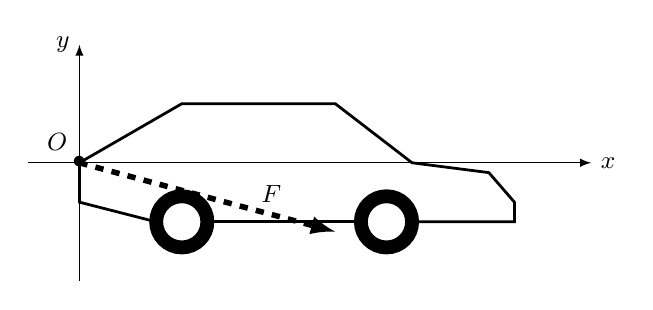
\begin{tikzpicture}[>=latex,yscale=0.5,xscale=0.65]
        \draw[->] (-1,0) -- (10,0) node[right] {\small $x$};
        \draw[->] (0,-3) -- (0,3) node[left] {\small $y$};
        \draw[line width=5pt] (2,-1.5) ellipse (0.5 and 0.65) ++(4,0) ellipse (0.5 and 0.65);
        \draw[line width=1pt] (1.5,-1.5) -- (0,-1) -- (0,0) -- (2,1.5) -- (5,1.5) -- (6.5,0) -- (8,-0.25) -- (8.5,-1) -- (8.5,-1.5) -- (6.5,-1.5);
        \draw[line width=1pt] (2.5,-1.5)--(5.5,-1.5);
        \draw[line width = 2pt,dashed,->] (0,0) node {$\bullet$} node[above left] {\small $O$} -- (5,-1.75) node[pos=0.75,above] {\small $\vect F$};
    \end{tikzpicture}
\end{center}

\begin{enumerate}
    \item Décomposer le vecteur $\vect F$ en deux vecteurs $\vect{F}_x$ et $\vect F_y$ suivant les deux axes orthogonaux $(Ox)$ et $(Oy)$. Dessiner cette décomposition en deux vecteurs sur le dessin.
    \item Sans utiliser le produit scalaire, déterminer la norme de la force qui permet à la voiture d'avancer.
    \item Calculer alors le travail nécessaire pour faire avancer la voiture sur une distance de $10$ mètres.
\end{enumerate}\[*\]

\exo On considère un triangle $ABC$ quelconque.
\begin{enumerate}
    \item \'Ecrire en justifiant $\PS{BC}{BC}$ en fonction de $\norme{\vect{BC}}$.
    \item En utilisant le fait que $\vect{BC} = \vect{BA} + \vect{AC}$, démontrer la formule d'Al-Kashi :
        \[BC^2 = AB^2 + AC^2 - 2 \times AB \times AC \times \cos\left(\vect{AB}\pv\vect{AC}\right).\]
    \item Que se passe-t-il lorsque le triangle $ABC$ est rectangle en $A$ ?
    \item Dessiner un triangle $ABC$ tel que $BC = 5~cm$, $AC = 7~cm$ et $AB = 4~cm$.\par
        Utiliser la formule d'Al-Kashi pour calculer la mesure des trois angles du triangle. Arrondir au degré près.
\end{enumerate}\[*\]

\exo Un enfant est situé en haut d'une piste de ski. Il se laisse glisser en ligne droite face à la pente d'un point $A$ à un point $B$. La pente forme un angle de $\alpha$ degrés avec l'horizontale. L'enfant est matérialisé par un point $E$.
\begin{enumerate}
    \item Réaliser un schéma modélisant la situation.
    \item Tous les frottements sont négligés : l'enfant n'est donc soumis qu'à deux actions mécaniques : le poids $\vect P$ et la réaction du sol $\vect R$.\par
        Compléter le schéma en dessinant ces deux vecteurs.
    \item Quel est le travail de la force $\vect R$ dans ce déplacement ? Justifier la réponse.
    \item Expliquer pourquoi $\left(\vect{P}\pv\vect{AB}\right) = 90 - \alpha$. En déduire le signe de $\cos\left(\vect{P}\pv\vect{AC}\right)$.
    \item Sachant que $\norme{\vect P} = mg$, écrire le travail $\PS{P}{AB}$ en fonction de $m$, $g$, $\alpha$ et $AB$. Quel est le signe de ce travail ? Interpréter.
    \item La variation de l'énergie cinétique du système entre $A$ et $B$ est égale à la somme des travaux des actions mécaniques qui agissent sur le système. On a donc :
        \[\PS{P}{AB} + \PS{R}{AB} = \dfrac 1 2 m v^2.\] Le nombre $v$ est la vitesse acquise par l'enfant lorsqu'il arrive en $B$ ; elle est exprimée en $m\cdot s^{-1}$.\par
        En utilisant les données ci-dessous, déterminer l'arrondie à l'unité de la vitesse acquise par l'enfant après s'être laissé glissé sur une distance de $20~m$ :
        \[\alpha = 9\degres \qq m = 25~kg \qetq g = 9,81~m\cdot s^{-1}.\]
\end{enumerate}
\end{document} 